\qs{Určete definiční obor funkce $f$, je-li dáno}{
	$$ f(x) = \frac{\arccos{\frac{2x - 11}{13}}}{\ln(16 - x^2)} $$
}

\defi{Definice funkce $\arccos$}{
	\begin{align*}
		f(x) &\coloneq \cos{x} \\
		f^{-1}(x) &\coloneq \arccos{x} \\
	\end{align*}
}

Naše funkce je omezená jak přirozeným logaritmem $\ln$, tak f-ci $\arccos$ a podmínkou že $ln$ nesmí jako nulové. Definiční obor funkce $f(x) = \ln{x}$ je $D(f) = (0, \infty)$, u funkce $g(x) = \arccos{x}$ je to $D(g) = \left< -1, 1 \right>$. 
Náš výraz $\left( 16 - x^2 \right)$ se proto nesí rovnat nule nebo negativnímu číslu. Horní výraz $\frac{2x - 11}{13}$ aby uspokojil f-ci $\arccos$ je omezený v intervalu $\left< -1,1 \right>$. Naši funkci si rozdělíme na dva problémy, od nich vyřešíme definiční obory a tyto výsledně sjednotíme (konjunkce). 

$$ f(x) = \frac{f}{g} $$

\begin{align}
	\ln{16 - x^2} &\neq 0 \\
	16 - x^2 > 0 &\wedge 16 - x^2 \neq 1\\
	-x^2 > -16 &\wedge -x^2 \neq -15 \\
	x^2 < 16 &\wedge x \neq \sqrt{15} \\
	x < 4 &\wedge x \neq \sqrt{15} \\
	D(g) &= (4, \infty) \setminus \{ \sqrt{15} \}
\end{align}

\begin{align}
	-1 &\leq 2x - 11 \leq 1 \\
	-1 &\leq 2x - 11 \\
	10 &\leq 2x \\
	5 &\leq x \\
	2x - 11 &\leq 1 \\
	2x &\leq 12 \\
	x &\leq 6 \\
	D(f) &= \left(-\infty, 6\right> \cap \left<5, \infty \right) = \left<5, 6\right>
\end{align}

Definiční obor naší f-ce $f$ je 
$$
D(f) = \left< 5,6 \right> \cap \left( 4,\infty \right) \setminus \{\sqrt{15}\} \rightarrow 
\left( 4, 6 \right> \setminus \{ \sqrt{15} \}
$$

\begin{center}
\textit{Graf funkce $f(x) \coloneq \cos{x}$ její inverzní funkce $f^{-1}(x) \coloneq \arccos{x}$}
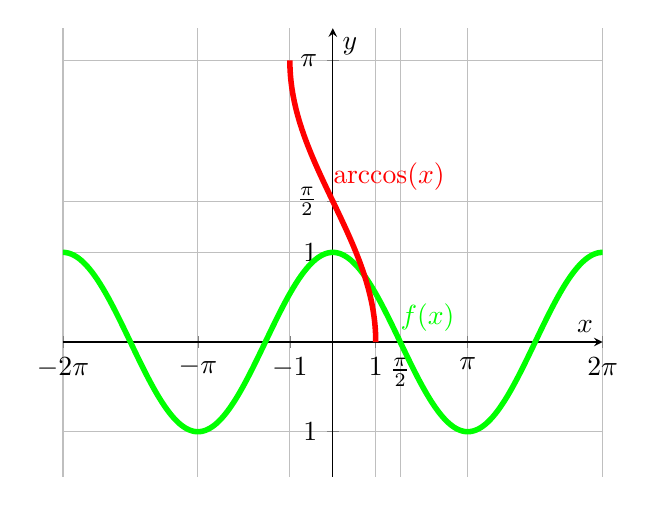
\begin{tikzpicture}
    \begin{axis}[
        axis lines=middle,
        samples=1000,
        restrict x to domain=-12:12,
        restrict y to domain=-10:10,
        xlabel=$x$,
        ylabel=$y$,
        xmin=-2*pi,
        xmax=2*pi,
        ymin=-1.5,
        ymax=3.5,
        xmajorgrids=true,
        ymajorgrids=true,
		xtick={-2*pi, -pi, -1, 1, pi/2, pi, 2*pi},
		xticklabels={$-2\pi$, $-\pi$, $-1$, $1$, $\frac{\pi}{2}$, $\pi$, $2\pi$},
		ytick={-1, 1, pi/2, pi},
		yticklabels={$1$, $1$, $\frac{\pi}{2}$, $\pi$},
    ]
    
    % Plot cosine function
    \addplot[line width=2pt,color=green,domain=-2*pi:2*pi]{cos(deg(x))}
        node[right,pos=0.6]{$f(x)$};

    % Plot arccosine function
    \addplot[line width=2pt,color=red,domain=-1:1]{ ( acos(x) ) * (pi/180) }
        node[right,pos=0.4]{$\arccos(x)$};
    
    \end{axis}
\end{tikzpicture}
\end{center}

\begin{center}
\textit{}
    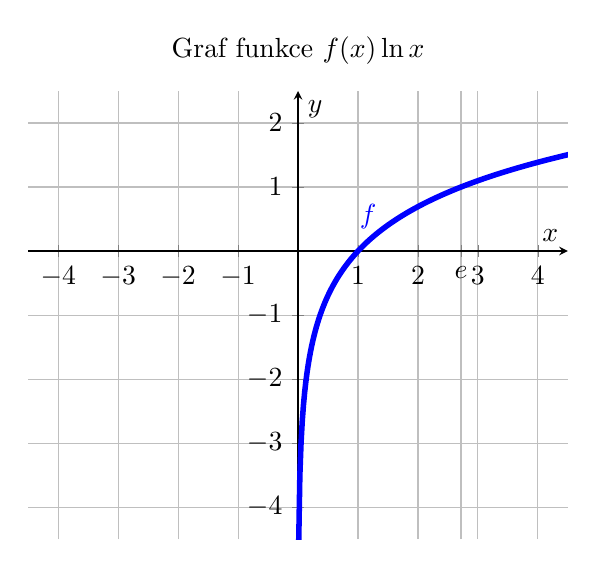
\begin{tikzpicture}
        \begin{axis}[
            axis lines=middle,
            restrict x to domain=-6:6,
            restrict y to domain=-10:20,
            xmin=-4.5,
            xmax=4.5, 
            ymin=-4.5,
            ymax=2.5, 
            xlabel=$x$,
            ylabel=$y$,
			title=Graf funkce $f(x) \coloneq \ln{x}$,
			xtick={-4, -3, -2, -1, 1, 2, e, 3, 4},
			xticklabels={$-4$, $-3$, $-2$, $-1$, $1$, $2$, $e$, $3$, $4$},
			ytick={-4,-3,-2,-1,1,2},
			yticklabels={$-4$,$-3$,$-2$,$-1$,$1$,$2$},
            % xticklabel style={anchor=south west},
			ymajorgrids=true,
            xmajorgrids=true,
		]
        % \begin{axis}[xmin=-10, xmax=10, ymin=-10, ymax=10, axis lines = middle]
            \addplot[blue, samples=500, line width=2pt]{ ln(x) }
            node[above, pos=0.55]{$f$};
        \end{axis}
    \end{tikzpicture}
\end{center}

